%%%%%%%%%%%%%%%%%%%%%%%%%%%%%%%%%%%%%%%%%%%%%%%%%%%%%%%
% MatPlotLib and Random Cheat Sheet
%
% Edited by Michelle Cristina de Sousa Baltazar
% Updated by Bella Nicholson
%
% http://matplotlib.org/api/pyplot_summary.html
% http://matplotlib.org/users/pyplot_tutorial.html
%
%%%%%%%%%%%%%%%%%%%%%%%%%%%%%%%%%%%%%%%%%%%%%%%%%%%%%%%

\documentclass[a4paper]{article}
\usepackage[landscape]{geometry}
\usepackage{url}
\usepackage{multicol}
\usepackage{amsmath}
\usepackage{amsfonts}
\usepackage{tikz}
\usetikzlibrary{decorations.pathmorphing}
\usepackage{amsmath,amssymb}
\usepackage{mathtools}
\usepackage{amsthm, amsmath, amssymb, amsfonts}
\usepackage{enumitem}
\usepackage{fontawesome}
\usepackage[hidelinks]{hyperref}
\usepackage{xcolor}

%%%%%%%%%%%%%%
% Table formatting
%%%%%%%%%%%%%%
% To make a pretty table
% Table colors setup
\definecolor{tableoutlinecolor}{HTML}{A599E9} 
\definecolor{rowcolor1}{HTML}{2D2B55} % Red
\definecolor{rowcolor2}{HTML}{1E1E3F} % Green

\usepackage{colortbl}
%\rowcolors{1}{rowcolor1}{rowcolor2}
\usepackage{tabularx}
%%%%%%%%%%%%%%

%\title{Git Cheat Sheet}
\usepackage[english]{babel}
\usepackage[utf8]{inputenc}
\usepackage{bm}

% Insert nice figures in 
\usepackage{graphicx}
\usepackage{caption}
\captionsetup{
	font=tiny,
}


\newcommand{\pd}[2]{\frac{\partial #1}{\partial #2}}
\newcommand{\loss}[0]{\mathcal{L}}
\newcommand{\chain}[3]{\frac{\partial #1}{\partial #2}\frac{\partial #2}{\partial #3}}
\newcommand{\eq}[1]{\begin{equation*}\begin{split}#1\end{split}\end{equation*}}
\newcommand{\coderef}[0]{Please find the implementation in the folder with the code files.}
\newcommand{\TODO}[1]{\textbf{\textcolor{red}{#1}}}


%%%%%%%%%%%%%%
% Shades of purple colors
%%%%%%%%%%%%%%

% Define colors
\definecolor{background}{HTML}{2D2B55}
\definecolor{darkbackground}{HTML}{1E1E3F}
\colorlet{boxcolor}{background!90}
\definecolor{textcolor}{HTML}{FFFFFF} %{FFFFFF}  %{B362FF}
\definecolor{goldenyellow}{HTML}{FAD000}  % FFEE80
\definecolor{lightyellow}{HTML}{FFEE80} 
\definecolor{lightpurple}{HTML}{A599E9}
\definecolor{brightpurple}{HTML}{B362FF} %{B362FF} % 4D21FC
\definecolor{brightgreen}{HTML}{3AD900} %A5FF90,  3AD900
\colorlet{green}{brightgreen!65}
\definecolor{icyblue}{HTML}{9EFFFF}
\definecolor{deeppink}{HTML}{FF628C}
\definecolor{icypink}{HTML}{FB94FF}
\definecolor{paleyellow}{HTML}{FAEFA5}
\definecolor{orange}{HTML}{FF9D00}
\definecolor{red}{HTML}{EC3A37}
\colorlet{linkcolor}{lightyellow}

% Apply color selection to document
\pagecolor{background}
\color{textcolor}
\hypersetup{
	colorlinks=true,
	linkcolor=linkcolor,
	urlcolor=linkcolor,
}

%%%%%%%%%%%%%%
%     Make a footer
%%%%%%%%%%%%%%
\geometry{left=0.25cm,right=0.25cm,top=0.25cm,bottom=0.6cm, footskip=0pt}
%\setlength{\footskip}{0pt}
%\textheight=600pt
\usepackage{fancyhdr}
\usepackage[absolute,overlay]{textpos}
\pagestyle{fancy}

\fancyfoot{}  % Clear all footer fields
\fancyfoot[R]{ 
	\textcolor{lightpurple}{\small{
	\vspace{-3cm}
	\href{https://github.com/bellanich}{\faGithub{} {bellanich}} \hspace{0.3cm}
	\href{https://www.linkedin.com/in/bella-nicholson}{\faLinkedinSquare{} {bella-nicholson}}
	}}
}
%%%%%%%%%%%%%%


%%%%%%%%%%%%%%%
% Make pretty in-line code
%%%%%%%%%%%%%%%
\usepackage{listings}
\usepackage[T1]{fontenc}
% Define bash command styling for using in textbox
\lstdefinestyle{inlinecode}{
	basicstyle=\ttfamily\color{brightpurple},
	keywordstyle=\bfseries,
	breaklines=true,
	keepspaces=true,
	frame=single,
}
\newcommand{\inlinebash}[1]{\lstinline[style=inlinecode]{#1}}

% Define bash command styling for using in table
\lstdefinestyle{tablebash}{
	basicstyle=\ttfamily\color{darkbackground},
	keywordstyle=\bfseries,
	breaklines=true,
	keepspaces=true,
	frame=single,
	literate=%
	{"}{\textquotedbl}1
	{'}{\textquotesingle}1
}
\newcommand{\tablebash}[1]{{\lstinline[style=tablebash]{#1}}}
%%%%%%%%%%%%%%%


\parindent0pt
\parskip2pt


\begin{document}


%%%%%%%%%%%%%%%
%      TITLE
%%%%%%%%%%%%%%%
\begin{center}
	\textcolor{lightpurple}{
		\textbf{\LARGE{Git Cheat Sheet}}\\
	}
\end{center}
%%%%%%%%%%%%%%%



%%%%%%%%%%%%%%%
%      Cheat Sheet Body
%%%%%%%%%%%%%%%
\footnotesize
\begin{multicols*}{3}

\tikzstyle{mybox} = [draw=black, fill=white, very thick,
    rectangle, rounded corners, inner sep=10pt, inner ysep=10pt]
\tikzstyle{fancytitle} =[fill=black, text=white, font=\bfseries]



\colorlet{outlinecolor}{icypink}

\begin{tikzpicture}
	\node [mybox, fill=boxcolor, draw=outlinecolor] (box){%
		\begin{minipage}{0.3\textwidth}
			\vspace{0.1cm}
			\underline{Source control} is the practice of tracking and managing changes to code. There are two types:
			\begin{enumerate}
				\item In \textcolor{outlinecolor}{centralized source control}, a centralized server acts as the ultimate source of truth for a collection of versioned files. 
				\begin{itemize}
					\item \textit{Implications.} An internet connection to the central server is required for most basic operations.
					\item \textit{Examples.} \href{https://subversion.apache.org}{Subversion}, \href{https://cvs.nongnu.org}{CVS}
				\end{itemize}
				\item \textcolor{outlinecolor}{Distributed or decentralized source control} doesn't require a central source of truth and allows for most operations to be local.
				\begin{itemize}
					\item \textit{Implications.} You can work independently of an internet connection.
					\item \textit{Examples.} Git, Mercurial (Hg)
				\end{itemize}
			\end{enumerate}
			\vspace{-3mm}
%			\begin{itemize}[leftmargin=4mm]
%				\setlength\itemsep{0.0em}
%				\item Neural Network is a directed acyclic graph
%				% \item Every module can be expressed by $a=h(x;w)$
%				\item Use loss function that matches output distribution to improve numerical stability and make gradients larger
%				\item Input and output distribution of every module should be the same to prevent inconsistent behavior and harder learning
%			\end{itemize}
%			\underline{Backprop}: chain rule $\pd{z}{x_i}=\sum_j \chain{z}{y_j}{x_i}$, $\nabla_{\bm{x}} \bm{z} = \left(\pd{\bm{y}}{\bm{x}}\right)^T \cdot \nabla_{\bm{y}} \bm{z}$
%			\vspace{-1mm}
%			\begin{enumerate}[leftmargin=4mm, label=\arabic*.]
%				\setlength\itemsep{0.2em}
%				\item Compute forward: $a^{(l)} = h^{(l)}\left(x^{(l)}\right)$, $x^{(l+1)}=a^{(l)}$
%				\item Compute reverse: $\pd{\loss}{a^{(l)}} = \left(\pd{a^{(l+1)}}{x^{(l+1)}}\right)^T \cdot \pd{\loss}{a^{(l+1)}}$\\
%				$\pd{\loss}{\theta^{(l)}} = \pd{a^{(l)}}{x^{(l+1)}} \cdot \left(\pd{\loss}{a^{(l)}}\right)^T$
%				\item Update params: $\theta^{(l)}_{t+1} = \theta^{(l)}_{t}-\eta \nabla_{\theta_t^{(l)}}\loss$
%			\end{enumerate}
		\end{minipage}
	};
	\node[fancytitle, right=10pt, fill=outlinecolor, text=black, draw=outlinecolor, rounded corners] at (box.north west) {History of Git};
\end{tikzpicture}
\vspace{-2mm}


\colorlet{outlinecolor}{deeppink}

\colorlet{headercolor}{outlinecolor}
\colorlet{rowcolor1}{outlinecolor!70}
\colorlet{rowcolor2}{outlinecolor!50}

\begin{tikzpicture}
	\node [mybox, fill=boxcolor, draw=outlinecolor] (box){%
		\begin{minipage}{0.3\textwidth}
			\vspace{0.1cm}
			\textcolor{outlinecolor}{A repository} is a collection of version controlled files that are kept together. This includes \textbf{(a)} all the files related to a specific project/application, \textbf{(b)} the history of changes, and \textbf{(c)} any special configurations. \\
			
			\vspace{-1mm}
			\underline{Git states}: Git has \href{https://git-scm.com/book/en/v2/Getting-Started-What-is-Git%3F}{three \textbf{local} states}.
			\begin{enumerate}
				\item The \textcolor{outlinecolor}{working directory state} holds all the project or application files. These files may or may not be managed by Git, but Git is aware of them.
				\item The \textcolor{outlinecolor}{staging area state} or \textcolor{outlinecolor}{Git index state} is holding area for the queue of changes to be included in your next commit.
				\item The \textcolor{outlinecolor}{local Git repository state}  is a hidden folder called \inlinebash{.git}, which contains your entire local commit history.
			\end{enumerate}
			Git also has a \textcolor{outlinecolor}{remote (repository) state}, which is just another repository with its own three internal states. A specific Git command is used to move files between these states. i.e., \\
			
			\begin{minipage}{\textwidth}
				\centering
%				\vspace{-2mm}
				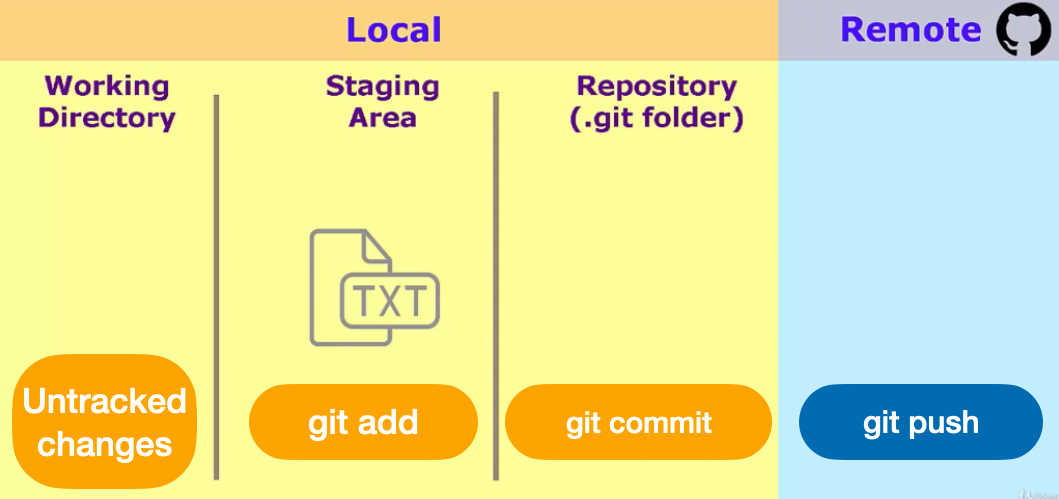
\includegraphics[width=0.5\textwidth]{images/git_stages.png}
				\vspace{-2mm}
				\captionof{figure}{Git states and associated commands. \href{https://www.udemy.com/course/git-complete/}{ \faLink{}  Source}}
			\end{minipage}
			\vspace{2mm}
			
			\underline{Tracking}: A \textcolor{outlinecolor}{tracked file}  is any file that Git is aware of and is actively tracking. In other words, any files that aren't new.
			
	
					
		\vspace{-3mm}
		\end{minipage}
	};
	\node[fancytitle, right=10pt, fill=outlinecolor, text=background, draw=outlinecolor, rounded corners] at (box.north west) {Git Theory};
\end{tikzpicture}
\begin{tikzpicture}
	\node [mybox, fill=boxcolor, draw=outlinecolor] (box){%
		\begin{minipage}{0.3\textwidth}
		\vspace{0.1cm}
		
		Here are useful commands to track new and existing files.
		\vspace{-2mm}
		\begin{center}
			\textcolor{background}{
				    \begin{tabularx}{\textwidth}{>{\columncolor{rowcolor1}}X|>{\columncolor{rowcolor2}}p{5cm}}
					\arrayrulecolor{boxcolor} % Table line color
					\rowcolor{headercolor} % Header row color
						\multicolumn{1}{c|}{\centering \textbf{Git Command}} & \multicolumn{1}{c}{\centering \textbf{Description}} \\ % Center the header text
					\hline % Add a horizontal line below the header row
					\rowcolor{rowcolor1} \tablebash{git ls-files} & Returns the list of files tracked by Git \\
					\rowcolor{rowcolor2} % Color of the second row
					\tablebash{git commit -am "commit message"} & Simultaneously add and commit a tracked file \\
					\rowcolor{rowcolor1} \tablebash{git add .} & Recursively add untracked files from current filepath location \\
				\end{tabularx}
			}
		\end{center}
		
			
		\end{minipage}
	};
	\node[fancytitle, right=10pt, fill=outlinecolor, text=background, draw=outlinecolor, rounded corners] at (box.north west) {Git Theory (2)};
\end{tikzpicture}

\vspace{-2mm}


\colorlet{outlinecolor}{orange}

\colorlet{headercolor}{outlinecolor}
\colorlet{rowcolor1}{outlinecolor!70}
\colorlet{rowcolor2}{outlinecolor!50}

\begin{tikzpicture}
	\node [mybox, fill=boxcolor, draw=outlinecolor] (box){%
		\begin{minipage}{0.3\textwidth}
			\vspace{0.1cm}
			\underline{Installation}: Depends on your OS.
			\begin{itemize}
				\item \textit{MacOS.} Normally, it's pre-installed. Otherwise, use command line developer tools to install it.
				\item \textit{WindowsOS.} Install the open source \href{https://gitforwindows.org}{Git for Windows Project}. Make sure to execute your Git commands from the \textcolor{outlinecolor}{Git Bash}.
			\end{itemize}
			
			\underline{Configure \& initialize}: You need to tell Git who you are and where the remote repository hosting platform is.
			\vspace{-2mm}
			\begin{center}
				\textcolor{background}{
					\begin{tabularx}{\textwidth}{>{\columncolor{rowcolor1}}X|>{\columncolor{rowcolor2}}p{4cm}}
						\arrayrulecolor{boxcolor} % Table line color
						\rowcolor{headercolor} % Header row color
						\multicolumn{1}{c|}{\centering \textbf{Git Command}} & \multicolumn{1}{c}{\centering \textbf{Description}} \\ % Center the header text
						\hline % Add a horizontal line below the header row
						\rowcolor{rowcolor1} \tablebash{git config --global user.name "bellanich"} & Set your global username \\
						\rowcolor{rowcolor2} % Color of the second row
						\tablebash{git config --global user.email "youremail@gmail.com"} & Set your global email \\
						\rowcolor{rowcolor1} \tablebash{git config --global --list} & Check your global configs \\
					\end{tabularx}
				}
			\end{center}
			
			\underline{Initialize your project}: Here's how to start a new Git project.
			\vspace{-2mm}
			\begin{center}
				\textcolor{background}{
					\begin{tabularx}{\textwidth}{>{\columncolor{rowcolor1}}X|>{\columncolor{rowcolor2}}p{4cm}}
						\arrayrulecolor{boxcolor} % Table line color
						\rowcolor{headercolor} % Header row color
						\multicolumn{1}{c|}{\centering \textbf{Git Command}} & \multicolumn{1}{c}{\centering \textbf{Description}} \\ % Center the header text
						\hline % Add a horizontal line below the header row
						\rowcolor{rowcolor1} \tablebash{git init my-project-name} & Initialize a new empty Git repository \\
						\rowcolor{rowcolor2} % Color of the second row
						\tablebash{git init} & Convert an existing dir into a Git project \\
						\rowcolor{rowcolor1} \tablebash{git clone git-project-url} & Initialize from your code hosting platform of choice \\
						\rowcolor{rowcolor2} \tablebash{git remote add origin git-project-url} & Add a remote reference to your local repository  \\
						\rowcolor{rowcolor1} \tablebash{git push origin main} & Force push to main branch (only do for initialization)  \\
					\end{tabularx}
				}
			\end{center}

			
%			\begin{minipage}{\textwidth}
%				\centering
%%				\vspace{-2mm}
%				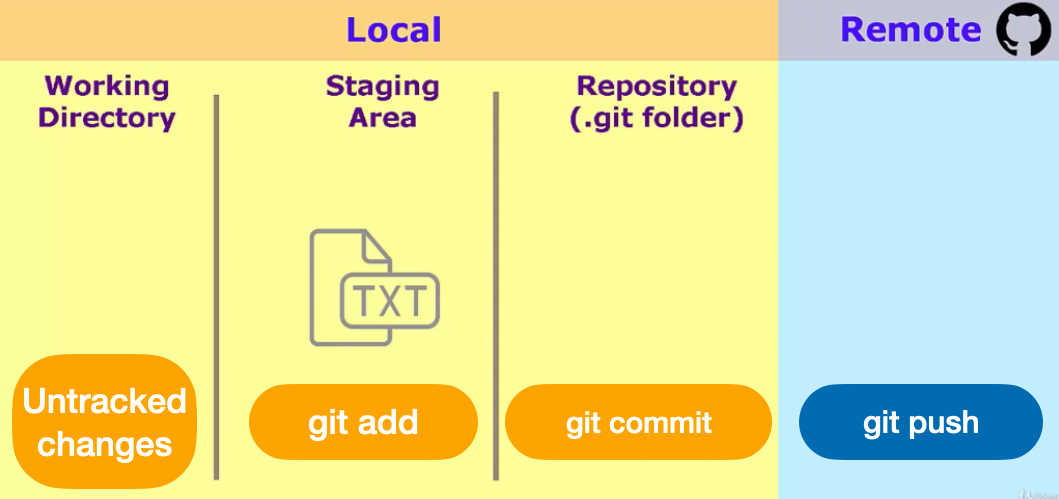
\includegraphics[width=0.5\textwidth]{images/git_stages.png}
%				\vspace{-2mm}
%				\captionof{figure}{Git states and associated commands. \href{https://www.udemy.com/course/git-complete/}{ \faLink{}  Source}}
%			\end{minipage}
			
		\end{minipage}
	};
	\node[fancytitle, right=10pt, fill=outlinecolor, text=background, draw=outlinecolor, rounded corners] at (box.north west) {Quick Start};
\end{tikzpicture}

\vspace{-3mm}


\colorlet{outlinecolor}{green}

\colorlet{headercolor}{outlinecolor}
\colorlet{rowcolor1}{outlinecolor!70}
\colorlet{rowcolor2}{outlinecolor!50}

\begin{tikzpicture}
	\node [mybox, fill=boxcolor, draw=outlinecolor] (box){%
		\begin{minipage}{0.3\textwidth}
			\vspace{0.1cm}
			\underline{Introduction}: Your \textcolor{outlinecolor}{Git commit history} is the chronological record of all commits ever made within your Git repository, where each commit is a snapshot of your project at a specific point in time. \\
			\vspace{-2mm}
			\begin{itemize}
				\item \textit{Implications.} The commit messages you make matter. We recommend writing \href{https://www.conventionalcommits.org/en/v1.0.0/}{conventional commits}.
			\end{itemize}
			
			A project's Git history is typically \textcolor{outlinecolor}{represented as a directed acyclic graph (DAG)} data structure.
			\vspace{-1mm}
	
		\end{minipage}
	};
	\node[fancytitle, right=10pt, fill=outlinecolor, text=background, draw=outlinecolor, rounded corners] at (box.north west) {Commit History};
\end{tikzpicture}


\begin{tikzpicture}
	\node [mybox, fill=boxcolor, draw=outlinecolor] (box){%
		\begin{minipage}{0.3\textwidth}
			\vspace{0.1cm}
	
			\underline{How does Git commit history work?} Git doesn't copying entire files in each commit. Rather, it uses a system of blobs and pointers.
			\begin{itemize}
				\item Git uses \href{https://www.thesslstore.com/blog/difference-sha-1-sha-2-sha-256-hash-algorithms/}{SHA-1 hashing} to create unique identifiers (hashes) for file content and stores
				\item The hashes are stored as \textcolor{outlinecolor}{blobs}  (\textcolor{outlinecolor}{b}inary \textcolor{outlinecolor}{l}arge \textcolor{outlinecolor}{ob}jects) in a database
				\item Git uses  pointers to reference the changes made to these blobs in its commit history 
			\end{itemize} 
			
			
			\underline{Search}: Here is how you can search through your Git history logs.
			
			\vspace{-2mm}
			\begin{center}
					\textcolor{background}{
							\begin{tabularx}{\textwidth}{>{\columncolor{rowcolor1}}X|>{\columncolor{rowcolor2}}p{4cm}}
									\arrayrulecolor{boxcolor} % Table line color
									\rowcolor{headercolor} % Header row color
									\multicolumn{1}{c|}{\centering \textbf{Git Command}} & \multicolumn{1}{c}{\centering \textbf{Description}} \\ % Center the header text
									\hline % Add a horizontal line below the header row
									\rowcolor{rowcolor1} \tablebash{git log --oneline --graph --decorate} & View your entire Git history in a user friendly way \\
									\rowcolor{rowcolor2} % Color of the second row
									\tablebash{git log --since="3 days ago"} & Search for all Git commits made in the last 3 days \\
									\rowcolor{rowcolor1} % New Row
									\tablebash{git log  -- your\_filename} & Get the history for only a specific file \\
									\rowcolor{rowcolor2} % New Row
									\tablebash{git log --follow -- your\_filename} & Include filename changes in your Git history search \\
									\rowcolor{rowcolor1} % New Row
									\tablebash{git show git\_commit\_hash} & See a given commit’s entire content, including: commit message, that commit’s git diff results, author, and date \\
								\end{tabularx}
						}
				\end{center}
				
				\vspace{-2mm}
				\underline{Compare}: You can what you have and haven't committed in Git. You can also compare different points in your commit history.
				
				\vspace{-2mm}
				\begin{center}
					\textcolor{background}{
						\begin{tabularx}{\textwidth}{>{\columncolor{rowcolor1}}X|>{\columncolor{rowcolor2}}p{4cm}}
							\arrayrulecolor{boxcolor} % Table line color
							\rowcolor{headercolor} % Header row color
							\multicolumn{1}{c|}{\centering \textbf{Git Command}} & \multicolumn{1}{c}{\centering \textbf{Description}} \\ % Center the header text
							\hline % Add a horizontal line below the header row
							\rowcolor{rowcolor1} \tablebash{git diff} & Compare staged and unstaged changes in your working directory to your last commit.  \\
							\rowcolor{rowcolor2} \tablebash{git diff -- your\_filename} & Only preview comparisons for a specific file   \\
							\rowcolor{rowcolor1} \tablebash{git diff --staged HEAD} & Review the (staged) changes about to be committed \\
							\rowcolor{rowcolor2} \tablebash{git diff commit\_hash1 commit\_hash2} & Compare two commits \\
							\rowcolor{rowcolor1} \tablebash{git diff local\_branchname origin/remote\_branchname} & Compare local and remote branches \\
						\end{tabularx}
					}
				\end{center}
			
			%			\begin{minipage}{\textwidth}
				%				\centering
				%%				\vspace{-2mm}
				%				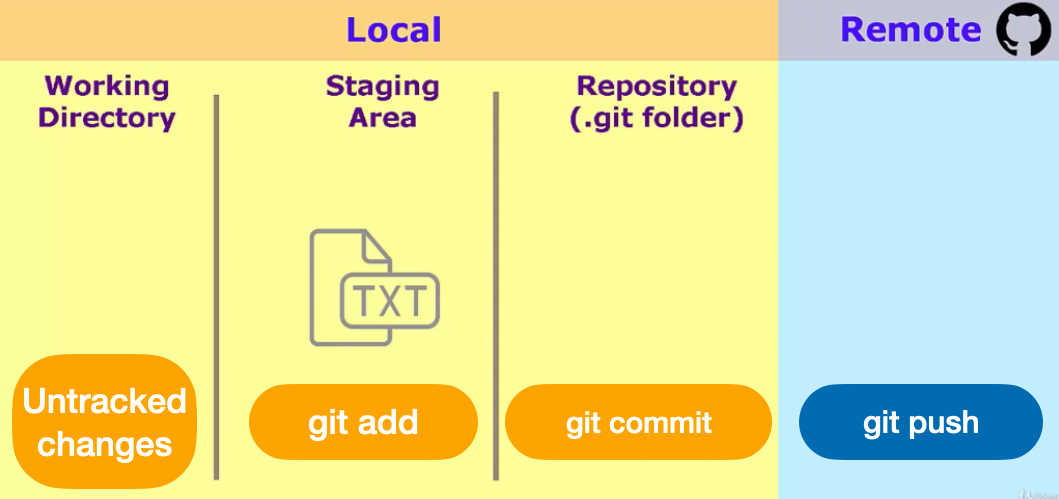
\includegraphics[width=0.5\textwidth]{images/git_stages.png}
				%				\vspace{-2mm}
				%				\captionof{figure}{Git states and associated commands. \href{https://www.udemy.com/course/git-complete/}{ \faLink{}  Source}}
				%			\end{minipage}
			
		\end{minipage}
	};
	\node[fancytitle, right=10pt, fill=outlinecolor, text=background, draw=outlinecolor, rounded corners] at (box.north west) {Commit History (2)};
\end{tikzpicture}


\end{multicols*}
%%%%%%%%%%%%%%%


\end{document}